%%%%%%%%%%%%Outline%%%%%%%%%%%%%%%%%%

% Section 4: \tool Design and Implementation

%%%
% message<overview of the section>
% xx

% Section 4.1: Design Principles

%%%
% message<preserve the existing safety boundary>
% userspace may propose rewrites
% every candidate goes through normal re-verification and re-JIT
% rejection leaves the running program unchanged

%%%
% message<preserve deployment transparency>
% always start from saved original bytecode rather than patching the installed image
% replace code in place for the same logical program
% after installation, execution still follows the ordinary JIT fast path

% Section 4.2: Design Challenges and Insights

%%%
% message<challenge: a live program has no stable rewrite baseline>
% verifier, fixups, and JIT already transform the installed form
% insight: save original bytecode at load time
% insight: always rebuild one whole-program candidate from that baseline

%%%
% message<challenge: richer code generation must remain safe and transparent>
% userspace, verifier, and JIT need one shared meaning for each added instruction family
% insight: use kinsn as the shared contract for validation and lowering
% build replacement off the fast path and publish it atomically in place

% Section 4.3: Implementation (introduce by components)

%%%
% message<architecture overview of \tool>
% follow the architecture workflow figure
% kernel keeps the ordinary fast path running and saves original bytecode at load time
% daemon reads a live program, rewrites a whole-program candidate using deployment facts, and sends it back
% kernel re-verifies, re-JITs, and replaces the native image in place for the same logical program
% userspace decides which candidate to try; kernel decides whether it is legal and safe

%%%
% message<userspace daemon>
% xxx

%%%
% message<kernel re-verification and re-JIT>
% xx

%%%
% message<safe publication>
% xx

%%%%%%%%%%%%Outline%%%%%%%%%%%%%%%%%%

\section{\tool Design and Implementation}
\label{sec:bpfrejit}

% [addressed] \note{Yusheng: rename section to \tool(bpfrejit) Design? You can frist say the design goal/princile 1, then say the challenge and our key insight again 2, then Merge Overall Workflow and Deplyment mode into one subsection as 3; }

% [addressed] \note{Yusheng: TODO, not need to describe mode here, it's just impl detail for test purpose. You can remove the Apply-all, describe the watch mode, and try to illustrate what it's different from traditional eBPF end to end deployment workflow in background}

Using kinsn as the optimization-facing program form introduced in Section~\ref{sec:kinsn}, \tool adds a post-load recompilation loop for live eBPF programs. Figure~\ref{fig:workflow} summarizes this loop. After a program is loaded and attached, the kernel keeps the ordinary JIT fast path running and saves the original bytecode as a stable baseline for future rewrites. A privileged userspace daemon discovers a live program, combines that baseline with deployment facts such as runtime profiles and stable values, and rewrites one whole-program candidate. The kernel then re-verifies that candidate, re-JITs it, and replaces the native image in place for the same logical program. This organization gives userspace control over which optimization or hardening candidate to try, while the kernel remains the final authority on legality and safety. The rest of this section states the design contract of this loop, identifies the two implementation constraints that shape it, and then walks through one optimization cycle in detail.

\begin{figure}[htbp]
  \centering
  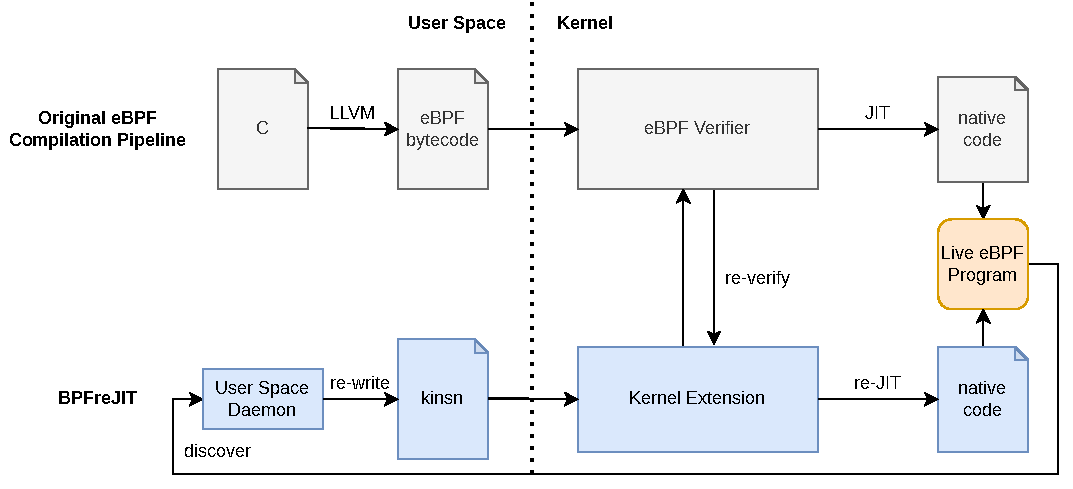
\includegraphics[width=\linewidth]{figures/sec-4-arch.drawio.pdf}
  \caption{Overview of \tool. The daemon reads a live program, rewrites a whole program in userspace, and sends it back to the kernel; the kernel re-verifies, re-JITs, and replaces the JIT code in place.}
  \label{fig:workflow}
\end{figure}


\subsection{Design Principles}
\label{sec:rejit-principles}

\noindent\textbf{Preserving the existing safety boundary.}
\tool does not bypass the kernel's existing admission path. Userspace may propose a rewritten program, but every candidate is submitted as a complete eBPF program and passes through the normal re-verification and re-JIT path before installation. The kernel therefore continues to enforce the same accept-or-reject safety boundary that already governs \texttt{BPF\_PROG\_LOAD}. If verification or recompilation fails, the candidate is discarded and the current live image remains in place. This fail-closed organization lets the daemon own rewrite construction without weakening the kernel's safety model.

\noindent\textbf{Preserving deployment transparency.}
\tool is designed to optimize already-loaded programs without changing how applications deploy them. Recompilation starts from the saved original bytecode rather than from the currently installed native image, and successful recompilation replaces code in place for the same logical program rather than detaching and reloading a new one. Existing applications, loaders, and attachment paths therefore continue to use the standard eBPF workflow. After installation, execution still follows the ordinary JIT fast path, so the framework adds no steady-state execution overhead beyond the one-time recompilation work.

\subsection{Implementation Challenges and Key Insights}
\label{sec:rejit-challenges}

There are two implementation challenges define the design of \tool.

\noindent\textbf{Challenge 1: Recovering a stable rewrite baseline.}
A live program is not a clean optimization input: verification, fixups, and JIT compilation have already transformed the installed form. \tool therefore saves the original bytecode at load time and restarts every recompilation round from that saved copy. This makes each round a whole-program reconstruction from one stable baseline, rather than an incremental patch over an already transformed image.

\noindent\textbf{Challenge 2: Supporting richer code generation without complicating kernel admission.}
Userspace needs a richer rewrite substrate than ordinary BPF idioms alone, but the kernel still needs one clear contract for checking and realizing rewritten code. \tool addresses this with kinsn: userspace introduces kinsn-backed realizations where beneficial, while the kernel validates and lowers them through the normal re-admission path. This extends post-load recompilation without turning the kernel JIT into a general optimizer.

\subsection{Userspace Rewrite Selection}
\label{sec:design-daemon}

\tool assigns rewrite selection to userspace. Whether a rewrite is worthwhile depends on deployment-specific information such as workload behavior, machine characteristics, and runtime values that only become visible after a program has been running. The daemon therefore decides when to revisit a live program and what candidate to try next, while the kernel remains responsible only for deciding whether that candidate is legal and safe.

The daemon always submits one rewritten whole program rather than incremental patches. Whole-program construction lets userspace compose interacting decisions before crossing the kernel boundary. When conditions change, the daemon can revisit the same live program by rebuilding a fresh candidate from the saved original bytecode and resubmitting it through the same kernel admission path. If the new candidate is rejected, the currently running program remains unchanged.
